%\documentclass[handout]{beamer} 
\documentclass[t,12pt,numbers,fleqn]{beamer}
%\documentclass[ignorenonframetext]{beamer}

\newif\ifquestions
%\questionstrue
\questionsfalse

\usepackage{pgfpages} 
\usepackage{hyperref}
\hypersetup{colorlinks=true,
    linkcolor=blue,
    citecolor=blue,
    filecolor=blue,
    urlcolor=blue,
    unicode=false}
\urlstyle{same}
\usepackage{listings}

\bibliographystyle{plain}

%\usetheme{Iimenau}

\useoutertheme{split} %so the footline can be seen, without needing pgfpages

%\pgfpagesuselayout{resize to}[letterpaper,border shrink=5mm,landscape]  %if this is uncommented, the hyperref links do not work

\mode<presentation>{}

\input{../def-beamer}

\newcommand{\topic}{10 Verification and Validation Continued}

%Title page information for 1D04 lectures slides

% Define year specific parameters - used in title page and footer

\newcommand{\season}{Fall} %use to switch between Winter and Fall
\newcommand{\instructor}{Dr.~Spencer Smith} %use to switch instructor
\newcommand{\instructSmall}{Dr.~Smith}
\newcommand{\yr}{2019}
\newcommand{\courseCode}{CAS 741, CES 741}
\newcommand{\courseTitle}{Development of Scientific Computing Software}

%\setbeamerfont{structure}{series=\bfseries}
%\usefonttheme[stillsansseriftext,stillsansserifmath]{serif}
\setbeamertemplate{navigation symbols}{} 
\setbeamertemplate{itemize item}[ball]

\title{
  {\normalsize \bf 
    \borange{\courseCode~(\courseTitle)\\ \season~\yr}}\\[2ex]
  {\Large \bf \topic}}

\author[Smith]{\instructor}

\institute{
  Faculty of Engineering,
  McMaster University}

\date{
\today
%January 2011\\
\bc
  \includegraphics[scale = 0.2, keepaspectratio]
  {../mcmaster-logo-full-color.jpg}
\ec
}

\renewcommand{\borange}[1] %orange is too hard to read
{
   \bred{#1}
}

\begin{document}

\input{../footline}

%%%%%%%%%%%%%%%%%%%%%%%%%%%%%%%%%%%%%%%%%%%%%%%%%%%%%%

\begin{frame}
\frametitle{Verification and Validation Continued}

\bi
\item Administrative details
\item Questions?
\ei
\end{frame}

%%%%%%%%%%%%%%%%%%%%%%%%%%%%%%%%%%%%%%%%%%%%%%%%%%%%%%

\begin{frame}
\frametitle{Administrative Details}

\bi
\item GitHub issues for colleagues
\bi
\item Assigned 1 colleague (see \texttt{Repos.xlsx} in repo)
\item Provide at least 5 issues on their SRS
\ei
\item Reading week, no 741 classes
\item V\&V template updated in repo
\ei

\end{frame}

%%%%%%%%%%%%%%%%%%%%%%%%%%%%%%%%%%%%%%%%%%%%%%%%%%%%%%

\begin{frame}
\frametitle{Administrative Details: Deadlines}
~\newline
\begin{tabular}{l l l}
\textbf{SRS Issues} & Reading week & Oct 10\\
\textbf{V\&V Present} & Week 06 & Week of Oct 16\\
\textbf{V\&V Plan} & Week 07 & Oct 25\\
MG Present & Week 08 & Week of Oct 30\\
MG & Week 09 & Nov 8\\
MIS Present & Week 10 & Week of Nov 13\\
MIS & Week 11 & Nov 22\\
Impl.\ Present & Week 12 & Week of Nov 27\\
Final Documentation & Week 13 & Dec 6\\
\end {tabular}

\end{frame}

%%%%%%%%%%%%%%%%%%%%%%%%%%%%%%%%%%%%%%%%%%%%%%%%%%%%%%

\begin{frame}
\frametitle{Administrative Details: Presentation Schedule}

\bi
\item V\&V Present
\bi
\item \textbf{Tuesday: Steven, Alexandre P., Alexander S.}
\item \textbf{Friday: Geneva, Jason, Yuzhi}
\ei
\item MG Present
\bi
\item Tuesday: Xiaoye, Shusheng, Devi, Keshav, Alex P, Paul
\item Friday: Yuzhi, Jason, Geneva, Alex S, Isobel, Steven
\ei
\item MIS Present
\bi
\item Tuesday: Isobel, Keshav, Paul
\item Friday: Shusheng, Xiaoye, Devi
\ei
\item Impl.\ Present
\bi
\item Tuesday: Alexander S., Steven, Alexandre P.
\item Friday: Jason, Geneva, Yuzhi
\ei
\ei

\end{frame}

%%%%%%%%%%%%%%%%%%%%%%%%%%%%%%%%%%%%%%%%%%%%%%%%%%%%%%

\begin{frame}
\frametitle{Questions?}
\begin{itemize}
\item Questions about SRS?
\item Questions about V\&V?
\end{itemize}
\end{frame}

%%%%%%%%%%%%%%%%%%%%%%%%%%%%%%%%%%%%%%%%%%%%%%%%%%%%%%

\begin{frame}
\frametitle{White-box Testing}

\begin{itemize}
\item \structure{Intuitively, after running your test suites, what percentage of
    the lines of code in your program should be exercised?}
\end{itemize}

\end{frame}

%%%%%%%%%%%%%%%%%%%%%%%%%%%%%%%%%%%%%%%%%%%%%%%%%%%%%%

\begin{frame}
\frametitle{White-box Coverage Testing}

\begin{itemize}
\item (In)adequacy criteria - if significant parts of the program structure are not tested, testing is inadequate
\item Control flow coverage criteria
\begin{itemize}
\item Statement coverage
\item Edge coverage
\item Condition coverage
\item Path coverage
\end{itemize}
\end{itemize}
Examples that follow are from \cite{GhezziEtAl2003}
\end{frame}

%%%%%%%%%%%%%%%%%%%%%%%%%%%%%%%%%%%%%%%%%%%%%%%%%%%%%%

\begin{frame}
\frametitle{Statement-Coverage Criterion}

\begin{itemize}
\item Select a test set $T$ such that every elementary statement in $P$ is
  executed at least once by some $d$ in $T$
\item An input datum executes many statements - try to minimize the number of
  test cases still preserving the desired coverage
\end{itemize}

\end{frame}

%%%%%%%%%%%%%%%%%%%%%%%%%%%%%%%%%%%%%%%%%%%%%%%%%%%%%%

\begin{frame}
\frametitle{Example}

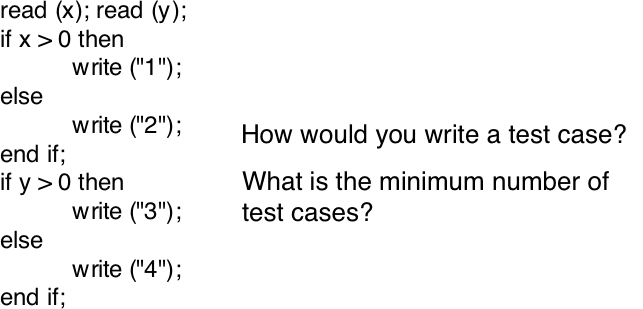
\includegraphics[scale=0.5]{../Figures/ExampleStatementCoverageOnlyCode.png}

\end{frame}

%%%%%%%%%%%%%%%%%%%%%%%%%%%%%%%%%%%%%%%%%%%%%%%%%%%%%%

\begin{frame}
\frametitle{Example}

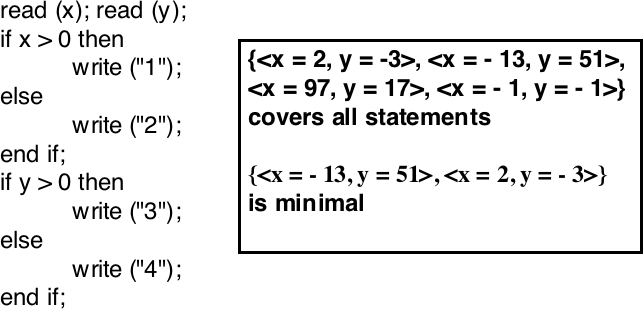
\includegraphics[scale=0.5]{../Figures/ExampleStatementCoverage.png}

\end{frame}

%%%%%%%%%%%%%%%%%%%%%%%%%%%%%%%%%%%%%%%%%%%%%%%%%%%%%%

\begin{frame}
\frametitle{Weakness of the Criterion}

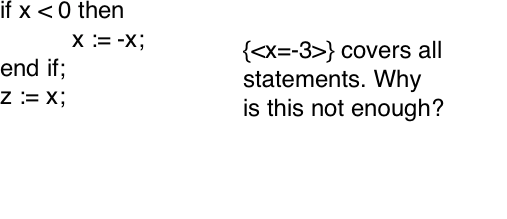
\includegraphics[scale=0.6]{../Figures/WeaknessStatementCoverageOnlyCode.png}

\end{frame}

%%%%%%%%%%%%%%%%%%%%%%%%%%%%%%%%%%%%%%%%%%%%%%%%%%%%%%

\begin{frame}
\frametitle{Weakness of the Criterion}

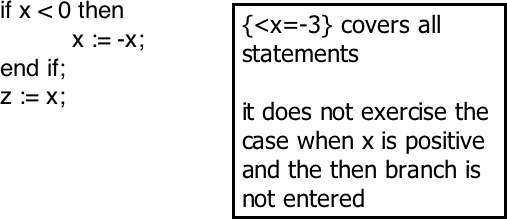
\includegraphics[scale=0.6]{../Figures/WeaknessStatementCoverage.png}

\end{frame}

%%%%%%%%%%%%%%%%%%%%%%%%%%%%%%%%%%%%%%%%%%%%%%%%%%%%%%

\begin{frame}
\frametitle{Edge-Coverage Criterion}

\begin{itemize}
\item Select a test set $T$ such that every edge (branch) of the control flow is
  exercised at least once by some $d$ in $T$
\item This requires formalizing the concept of the control graph and how to construct it
\begin{itemize}
\item Edges represent statements
\item Nodes at the ends of an edge represent entry into the statement and exit
\end{itemize}
\end{itemize}

\end{frame}

%%%%%%%%%%%%%%%%%%%%%%%%%%%%%%%%%%%%%%%%%%%%%%%%%%%%%%

\begin{frame}
\frametitle{Control Graph Construction Rules}

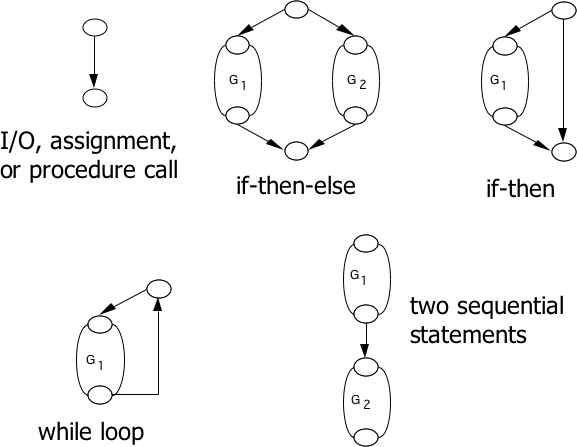
\includegraphics[scale=0.4]{../Figures/ControlGraphRules.png}

\end{frame}

%%%%%%%%%%%%%%%%%%%%%%%%%%%%%%%%%%%%%%%%%%%%%%%%%%%%%%

\begin{frame}
\frametitle{Simplification}

A sequence of edges can be collapsed into just one edge\\
~\newline

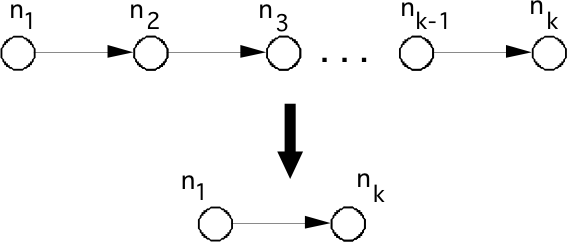
\includegraphics[scale=0.5]{../Figures/Simplification.png}

\end{frame}

%%%%%%%%%%%%%%%%%%%%%%%%%%%%%%%%%%%%%%%%%%%%%%%%%%%%%%

\begin{frame}
\frametitle{Example: Euclid's Algorithm}

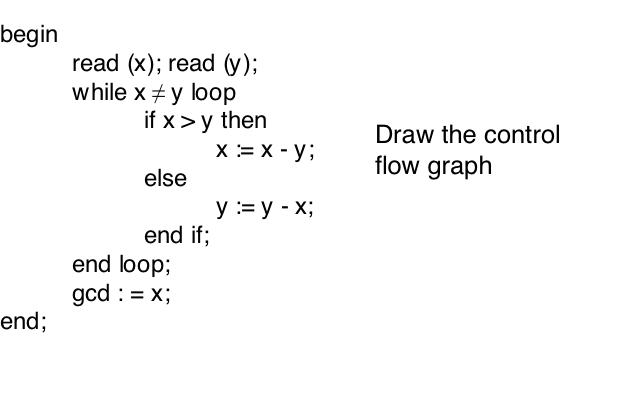
\includegraphics[scale=0.5]{../Figures/EuclidsAlgorithmNoGraph.png}

\end{frame}

%%%%%%%%%%%%%%%%%%%%%%%%%%%%%%%%%%%%%%%%%%%%%%%%%%%%%%

\begin{frame}
\frametitle{Example: Euclid's Algorithm}

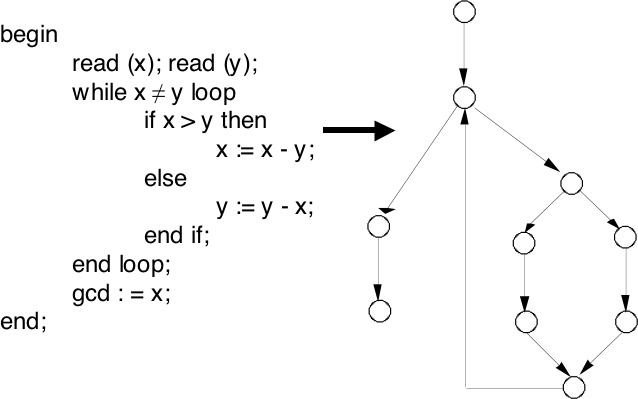
\includegraphics[scale=0.5]{../Figures/EuclidsAlgorithm.png}

\end{frame}

%%%%%%%%%%%%%%%%%%%%%%%%%%%%%%%%%%%%%%%%%%%%%%%%%%%%%%

\begin{frame}
\frametitle{Weakness}

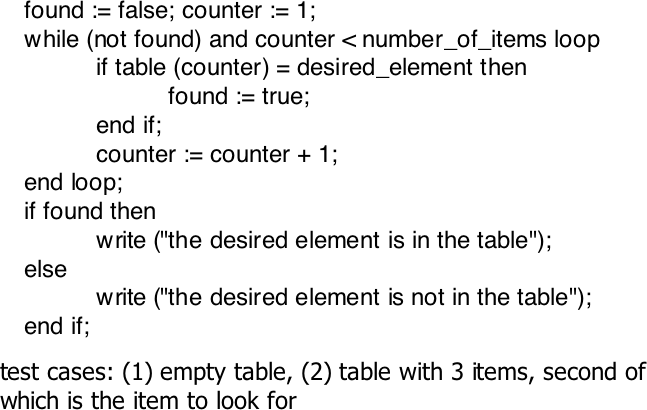
\includegraphics[scale=0.4]{../Figures/WeaknessEdgeCoverage.png}\\
\uncover<2->{\structure{Do not discover the error ($<$ instead of $\leq$)}}

\end{frame}

%%%%%%%%%%%%%%%%%%%%%%%%%%%%%%%%%%%%%%%%%%%%%%%%%%%%%%

\begin{frame}
%\frametitle{Alternative View of Condition Coverage}

\lstset{language=java,breaklines=true,showspaces=false,showstringspaces=false,breakatwhitespace=true}
\noindent \lstinputlisting{CondCovExample.java}

\end{frame}

%%%%%%%%%%%%%%%%%%%%%%%%%%%%%%%%%%%%%%%%%%%%%%%%%%%%%%

\begin{frame}
\frametitle{Condition-Coverage Criterion}

\begin{itemize}
\item Select a test set $T$ such that every edge of $P$'s control flow is traversed and all possible values of the
constituents of compound conditions are exercised at least once
\item This criterion is finer than edge coverage
\end{itemize}

\end{frame}

%%%%%%%%%%%%%%%%%%%%%%%%%%%%%%%%%%%%%%%%%%%%%%%%%%%%%%

\begin{frame}
\frametitle{Weakness}

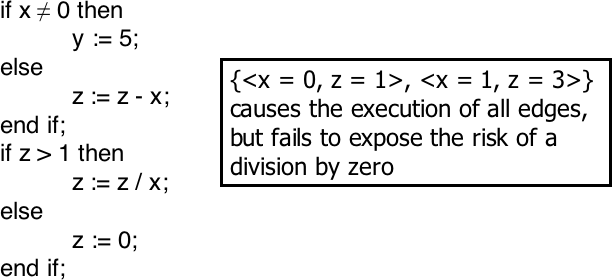
\includegraphics[scale=0.5]{../Figures/WeaknessConditionCoverage.png}

\end{frame}

%%%%%%%%%%%%%%%%%%%%%%%%%%%%%%%%%%%%%%%%%%%%%%%%%%%%%%

\begin{frame}
\frametitle{Path-Coverage Criterion}

\begin{itemize}
\item Select a test set $T$ that traverses all paths from the initial to the final node of $P$s control flow
\item It is finer than the previous kinds of coverage
\item However, number of paths may be too large, or even infinite (see while loops)
\item Loops
\begin{itemize}
\item Zero times (or minimum number of times)
\item Maximum times
\item Average number of times
\end{itemize}
\end{itemize}

\end{frame}

%%%%%%%%%%%%%%%%%%%%%%%%%%%%%%%%%%%%%%%%%%%%%%%%%%%%%%

\begin{frame}
\frametitle{The Infeasibility Problem}

\begin{itemize}
\item Syntactically indicated behaviours (statements, edges, etc.) are often impossible
\item Unreachable code, infeasible edges, paths, etc.
\item Adequacy criteria may be impossible to satisfy
\begin{itemize}
\item Manual justification for omitting each impossible test case
\item Adequacy ``scores'' based on coverage - example 95 \% statement coverage
\end{itemize}
\end{itemize}

\end{frame}

%%%%%%%%%%%%%%%%%%%%%%%%%%%%%%%%%%%%%%%%%%%%%%%%%%%%%%

\begin{frame}
\frametitle{Further Problem}

\begin{itemize}
\item What if the code omits the implementation of some part of the specification?
\item White box test cases derived from the code will ignore that part of the specification!
\end{itemize}

\end{frame}

%%%%%%%%%%%%%%%%%%%%%%%%%%%%%%%%%%%%%%%%%%%%%%%%%%%%%%

\begin{frame}
\frametitle{Testing Boundary Conditions}

\begin{itemize}

\item Testing criteria partition input domain in classes, assuming that behavior
  is ``similar'' for all data within a class
\item Some typical programming errors, however, just happen to be at the
  boundary between different classes
\begin{itemize}
\item Off by one errors
\item $<$ instead of $\leq$
\item equals zero
\end{itemize}
\end{itemize}

\end{frame}

%%%%%%%%%%%%%%%%%%%%%%%%%%%%%%%%%%%%%%%%%%%%%%%%%%%%%%

\begin{frame}
\frametitle{Criterion}

\begin{itemize}

\item After partitioning the input domain D into several classes, test the
  program using input values not only ``inside'' the classes, but also at their
  boundaries
\item This applies to both white-box and black-box techniques
\item In practice, use the different testing criteria in combinations
\end{itemize}

\end{frame}

%%%%%%%%%%%%%%%%%%%%%%%%%%%%%%%%%%%%%%%%%%%%%%%%%%%%%%

\begin{frame}
\frametitle{The Oracle Problem}

\structure{When might it be difficult to know the ``expected''
  output/behaviour?}

\end{frame}

%%%%%%%%%%%%%%%%%%%%%%%%%%%%%%%%%%%%%%%%%%%%%%%%%%%%%%

\begin{frame}
\frametitle{The Oracle Problem}

\begin{itemize}

\item Given input test cases that cover the domain, what are the expected
  outputs?
\item Oracles are required at each stage of testing to tell us what the right
  answer is
\item Black-box criteria are better than white-box for building test oracles
\item Automated test oracles are required for running large amounts of tests
\item Oracles are difficult to design - no universal recipe
\end{itemize}

\end{frame}

%%%%%%%%%%%%%%%%%%%%%%%%%%%%%%%%%%%%%%%%%%%%%%%%%%%%%%

\begin{frame}
\frametitle{The Oracle Problem Continued}

\begin{itemize}

\item Determining what the right answer should be is not always easy
\begin{itemize}
%\item Air traffic control system
\item Scientific computing
\item Machine learning
\item Artifical intelligence
\end{itemize}
\end{itemize}

\end{frame}

%%%%%%%%%%%%%%%%%%%%%%%%%%%%%%%%%%%%%%%%%%%%%%%%%%%%%%

\begin{frame}
\frametitle{The Oracle Problem Continued}

\structure{What are some strategies we can use when we do not have a test
  oracle?}

\end{frame}

%%%%%%%%%%%%%%%%%%%%%%%%%%%%%%%%%%%%%%%%%%%%%%%%%%%%%%

\begin{frame}
\frametitle{Strategies Without An Oracle}

\begin{itemize}

\item Using an independent program to approximate the oracle (pseudo oracle)
\item Method of manufactured solutions
\item Properties of the expected values can be easier than stating the expected
  output
\bi
\item \uncover<1->{\structure<1>{Examples?}}
\item \uncover<2->{List is sorted}
\item \uncover<2->{Number of entries in file matches number of inputs}
\item \uncover<2->{Conservation of energy or mass}
\item \uncover<2->{Expected trends in output are observed (metamorphic testing)}
\item \uncover<2->{etc.}
\ei
\end{itemize}

\end{frame}

%%%%%%%%%%%%%%%%%%%%%%%%%%%%%%%%%%%%%%%%%%%%%%%%%%%%%%

% \begin{frame}
% \frametitle{Analysis of Units}
% \begin{itemize}
% \item Dynamic testing of units is not the only option
% \item Static testing (analysis) includes the following
% \begin{itemize}
% \item Informal inspection
% \item Systematic inspection
% \item Code walkthroughs, data flow analysis
% \item Correctness proofs (for instance using pre and post conditions)
% \item Complexity measures
% \end{itemize}
% \end{itemize}
% \end{frame}

%%%%%%%%%%%%%%%%%%%%%%%%%%%%%%%%%%%%%%%%%%%%%%%%%%%%%%%%%%%%%%%%%%%%%%%%%%%%%

\begin{frame}
\frametitle{Challenges Specific to Scientific Computing}
\begin{itemize}
\item Unknown solution
\item Approximation of real numbers
\item Nonfunctional requirements
\item Parallel computation
\end{itemize}
\end{frame}

%%%%%%%%%%%%%%%%%%%%%%%%%%%%%%%%%%%%%%%%%%%%%%%%%%%%%%%%%%%%%%%%%%%%%%%%%%%%%

\begin{frame}
\frametitle{Mutation Testing for SC}
\begin{itemize}
\item Generate changes to the source code, called mutants, which become code faults
\item Mutants include changing an operation, modifying constants, changing the order of execution, etc.
\item The adequacy of a set of tests is established by running the tests on all generated mutants
\item Need to account for floating point approximations
\item See \cite{HookAndKelly2009}
\end{itemize}
\end{frame}

%%%%%%%%%%%%%%%%%%%%%%%%%%%%%%%%%%%%%%%%%%%%%%%%%%%%%%%%%%%%%%%%%%%%%%%%%%%%%

\begin{frame}
\frametitle{Specific SC V\&V Approaches}
Summary in \cite{Smith2016}
\begin{itemize}
\item Compare to closed-form solutions
\item Method of manufactured solutions \cite{Roache1998}
\item Interval arithmetic \cite{Hickey2001}
\item Convergence studies
\item Compare to other program (parallel testing)
\end{itemize}
\end{frame}

%%%%%%%%%%%%%%%%%%%%%%%%%%%%%%%%%%%%%%%%%%%%%%%%%%%%%%%%%%%%%%%%%%%%%%%%%%%%%

\begin{frame}
\frametitle{Specific SC V\&V NonFunctional}

\begin{itemize}
\item Installability, consider VMs
\item Portability, consider VMs, Docker, CI
\item Describe (rather than specify) impact of changing inputs
\bi
\item Accuracy
\item Performance
\item Relative comparison
\ei
\end{itemize}
\end{frame}

%%%%%%%%%%%%%%%%%%%%%%%%%%%%%%%%%%%%%%%%%%%%%%%%%%%%%%%%%%%%%%%%%%%%%%%%%%%%%

\begin{frame}
\frametitle{Validation Testing Report for PMGT}
\begin{itemize}
\item Prepared by Wen Yu
\item Do not know the correct solution, but know properties of the correct solution
\item Automated correctness validation tests
\begin{itemize}
\item The area of each element is greater than zero
\item The boundary of the mesh is closed
\item Vertices in a clockwise order
\item $nc + nv - ne = 1$
\item ...
\end{itemize}
\item Visual correctness validation tests
\begin{itemize}
\item No vertex outside the input domain
\item No vertex inside a cell
\item No dangling edges
\item All cells connected
\item  The mesh is conformal
\end{itemize}
\end{itemize}
\end{frame}

%%%%%%%%%%%%%%%%%%%%%%%%%%%%%%%%%%%%%%%%%%%%%%%%%%%%%%%%%%%%%%%%%%%%%%%%%%%%%

\begin{frame}
\frametitle{Validation Testing Report for PMGT (Continued)}
\begin{itemize}
\item List and description of test cases
\item Test cases are labelled and numbered
\item Traceability to SRS requirements
\item Traceability to MG
\item Summary of results
\item Analysis of results
\begin{itemize}
\item Focus on nonfunctional requirements
\item Speed
\end{itemize}
\end{itemize}
\end{frame}

%%%%%%%%%%%%%%%%%%%%%%%%%%%%%%%%%%%%%%%%%%%%%%%%%%%%%%%%%%%%%%%%%%%%%%%%%%%%%

\begin{frame}
\frametitle{Test Plan From BlankProjectTemplate}
\end{frame}

%%%%%%%%%%%%%%%%%%%%%%%%%%%%%%%%%%%%%%%%%%%%%%%%%%%%%%%%%%%%%%%%%%%%%%%%%%%%%

\begin{frame}[allowframebreaks]
\frametitle{References}

\bibliography{../../ReferenceMaterial/References}

\end{frame}

%%%%%%%%%%%%%%%%%%%%%%%%%%%%%%%%%%%%%%%%%%%%%%%%%%%%%%

\end{document}